Dado triângulo $ABC$ mostre como construir com régua e compasso um triângulo $A'B'C'$ de área
mínima com $C' \in AC$, $A' \in AB$ e $B' \in BC$ tal que $\angle B'A'C' = \angle BAC$ e $\angle A'C'B' = \angle AC B$.

\begin{center}
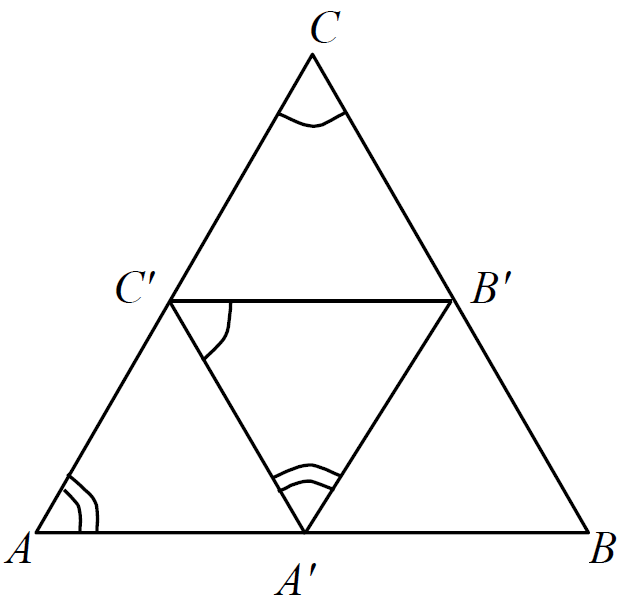
\includegraphics[width = 4cm]{figura.png}
\end{center}